\documentclass{report}

\usepackage[utf8]{inputenc}
\usepackage[T1]{fontenc}      
\usepackage[francais]{babel}
\usepackage{graphicx}
\usepackage{circuitikz}
\usepackage[squaren, Gray]{SIunits}
\usepackage{sistyle}
\usepackage[autolanguage]{numprint}
\usepackage{pgfplots}
\pgfplotsset{compat=1.9}
\usepackage{amsmath,amssymb,array}

\title{Projet 2 - Rapport de Pré-jury}
\author{Groupe 115.3}
\date{\today}

\begin{document}

\maketitle
\tableofcontents
<<<<<<< HEAD
=======
\makeatletter

\makeatother
>>>>>>> 2d850e6edead63f316960f05fdf38a9593db2a6f

\part{Introduction}

\part{Contenu du rapport}

\chapter{Fonctionnement et dimensionnement}

\documentclass{article}

\usepackage[utf8]{inputenc}
\usepackage[T1]{fontenc}      
\usepackage[francais]{babel}
\usepackage{graphicx}
\usepackage{circuitikz}
\usepackage[squaren, Gray]{SIunits}
\usepackage{sistyle}
\usepackage[autolanguage]{numprint}
\usepackage{pgfplots}
\pgfplotsset{compat=1.9}
\usepackage{amsmath,amssymb,array}
\usepackage[top=2.5cm,bottom=2.5cm,right=2.5cm,left=2.5cm]{geometry}
\usepackage{url} 
\usepackage{tabularx}
\DeclareMathOperator{\dist}{d}
\newenvironment{abstract-fr}
{
	\begin{center}
		\textbf{Résumé} \\[0.5cm]
	\end{center}
}
{}

\newenvironment{abstract-en}
{
	\begin{center}
		\textbf{Summary} \\[0.5cm]
	\end{center}
}
{}
% New command pour la modélisation mécanique, tri à effectuer
\newcommand\fv[1]{{\bf #1}} % free vector
\newcommand\fvd[1]{\dot{\bf #1}} % free vector derivated
\newcommand\fvdd[1]{\ddot{\bf #1}} % free vector derivated
\newcommand\fvr[1]{\mathring{\bf #1}} % free vector relatively derivated
\newcommand\fvrr[1]{\overset{\circ\circ}{\bf #1}} % free vector relatively derivated
\newcommand\uv[1]{{\bf\hat{ #1}}} % unit vector
\newcommand\ui{{\bf\hat{I}}} % unit vector I
\newcommand\uj{{\bf\hat{J}}} % unit vector J
\newcommand\uk{{\bf\hat{K}}} % unit vector K
\newcommand\wrt[2]{\ensuremath{\tensor*[_{ #1}]{ #2}{}}} % With Respect To
\newcommand\wtr[3]{\ensuremath{\tensor*[_{ #1}]{ #2}{^{ #3}}}} % With Two Respect
\newcommand\omegaf{{\bm \omega}}
\newcommand\omegafr{\mathring{\bm \omega}}
\newcommand\omegafd{\dot{\bm \omega}}
\newcommand\omegaft{\tilde{\bm \omega}}
\newcommand\omegaftr{\mathring{\tilde{\bm \omega}}}
\newcommand\omegat{\tilde{\omega}}
\newcommand\omegatd{\tilde{\dot{\omega}}}
\newcommand\ine{{\bf I}}
\newcommand\st{{\bf L}}
\newcommand\pst{{\bf M}}
\newcommand\lm{{\bf N}}
\newcommand\am{{\bf H}}
\newcommand\amd{\dot{\am}}
\newcommand\fo{{\bf F}}
\newcommand\po{\mathcal{P}}
\newcommand\xg{\ensuremath{\fv{R}}}
\newcommand\xgd{\ensuremath{\fvd{R}}}
\newcommand\xgdd{\ensuremath{\fvdd{R}}}
\newcommand\dvec[1]{\dot{\vec{ #1}}}
\newcommand\ddvec[1]{\ddot{\vec{ #1}}}
\newcommand\qp{\dot{q}}
\newcommand\dqp{\Delta \dot{q}}
\usepackage{url} 
\usepackage{hyperref}
\hypersetup{
    colorlinks,
    citecolor=black,
    filecolor=black,
    linkcolor=black,
    urlcolor=black
}

\begin{document}

\section{Dimensionnement du haut-parleur}
Après avoir réalisé quelques recherches sur les haut-parleurs, nous avons pu imaginer le dispositif idéal 
à réaliser. En tenant compte des différentes contraintes qui nous étaient imposées, voici les différents 
choix que nous avons effectués.

\subsection{Pour le boîtier}
Nous devions pouvoir faire varier les fréquences (voir annexe "Cahier des Charges"), ce qui signifie que nous ne 
pouvions pas faire un caisson trop petit. La taille du caisson influence le son restitué par le haut-parleur :
un volume trop petit ne restituerait pas les extrêmes graves. Effectivement, à de très basses 
fréquences, l'enceinte close va se comporter comme une raideur supplémentaire qui augmente la fréquence de
résonance\footnote{Fréquence pour laquelle la réponse du circuit est maximale}, et donc augmente la 
fréquence de coupure du passe-haut\cite{volume}. Nous avons finalement opté pour un boîtier cubique de 
$\unit{25}{\centi\meter}$ de côté, étant donné que ces dimensions avaient eu un très beau résultat lors 
d'un projet d'une année antérieure. Nous avions pensé placer un évent à l'avant du haut-parleur 
pour augmenter le rendement en profitant de l'onde arrière, mais c'était plus difficile à construire, et 
il aurait fallu que l'on accorde l'évent, de manière à exploiter l'onde arrière correctement. Nous nous 
sommes donc finalement limités à une charge\footnote{Manière de séparer les ondes avant et arrière.} dite "\textit{close}"\cite{close}.  

Afin d'améliorer un peu le boîtier, nous avons également pensé aux éléments suivants :

\begin{itemize}
	\item	Des pieds en caoutchouc : placer des pieds en caoutchouc sur le boîtier de notre haut-parleur
				permet de réduire les déplacements dûs aux vibrations du haut-parleur ;
	\item	Un matériau acoustiquement absorbant à l'intérieur du haut-parleur : le but d'un tel matériau
				dans un haut-parleur est de supprimer le court-circuit acoustique\cite{absorber}.
\end{itemize}

\subsection{Pour la membrane}
Nous avons opté pour une membrane de diamètre de $\unit{17}{\centi\meter}$. Nous avons choisi cette valeur afin 
d'avoir une membrane assez large, pour exploiter le mieux possible la taille du caisson. C'est également un
diamètre assez répandu dans le commerce\cite{tlhp}. Nous respectons donc les normes.
La profondeur de la membrane est de $\unit{6}{\centi\meter}$, comme pour la plupart des membranes de ce
diamètre\cite{tlhp}. La membrane est réalisée en papier. Afin d'éviter les difficultés de pliage, nous avons opté pour
du tissus tendu en guise de ressort. 

\begin{table}[!htb]
	\centering
	\begin{tabularx}{\textwidth}{|X|X|}
		\hline
			 \textbf{Caractéristique} & \textbf{Justification} \\
		\hline
			Volume du caisson : $\unit{25\times25\times25}{\centi\meter}$ & Possibilité de faire varier les fréquences.  \\
		\hline
			Matériau du caisson : Panneau de 	MDF
			d'épaisseur \unit{18}{\milli\meter} & Qualité, robustesse et coût. \\
		\hline
			Diamètre de membrane : \unit{17}{\centi\meter} & Avoir une membrane assez large pour exploiter le mieux possible la taille du caisson. \\
		\hline
			Profondeur de la membrane : \unit{6}{\centi\meter} & Déterminé en fonction du diamètre de la membrane. \\
		\hline
			Materiau membrane : papier et tissus & Rigidité et petite constante de raideur. \\
		\hline
			Masse surfacique du papier : \unit{200}{\gram\per\meter\squared} & Rigidité et coût. \\
		\hline
	\end{tabularx}
	\caption{Tableau récapitulatif.}
\end{table}

% Just here to fix rapport_prejury.tex
\end{document}


\documentclass{article}

\usepackage[utf8]{inputenc}
\usepackage[T1]{fontenc}      
\usepackage[francais]{babel}
\usepackage{graphicx}
\usepackage{circuitikz}
\usepackage[squaren, Gray]{SIunits}
\usepackage{sistyle}
\usepackage[autolanguage]{numprint}
\usepackage{pgfplots}
\pgfplotsset{compat=1.9}
\usepackage{amsmath,amssymb,array}
\usepackage[top=2.5cm,bottom=2.5cm,right=2.5cm,left=2.5cm]{geometry}
\usepackage{url} 
\usepackage{tabularx}
\DeclareMathOperator{\dist}{d}
\newenvironment{abstract-fr}
{
	\begin{center}
		\textbf{Résumé} \\[0.5cm]
	\end{center}
}
{}

\newenvironment{abstract-en}
{
	\begin{center}
		\textbf{Summary} \\[0.5cm]
	\end{center}
}
{}
% New command pour la modélisation mécanique, tri à effectuer
\newcommand\fv[1]{{\bf #1}} % free vector
\newcommand\fvd[1]{\dot{\bf #1}} % free vector derivated
\newcommand\fvdd[1]{\ddot{\bf #1}} % free vector derivated
\newcommand\fvr[1]{\mathring{\bf #1}} % free vector relatively derivated
\newcommand\fvrr[1]{\overset{\circ\circ}{\bf #1}} % free vector relatively derivated
\newcommand\uv[1]{{\bf\hat{ #1}}} % unit vector
\newcommand\ui{{\bf\hat{I}}} % unit vector I
\newcommand\uj{{\bf\hat{J}}} % unit vector J
\newcommand\uk{{\bf\hat{K}}} % unit vector K
\newcommand\wrt[2]{\ensuremath{\tensor*[_{ #1}]{ #2}{}}} % With Respect To
\newcommand\wtr[3]{\ensuremath{\tensor*[_{ #1}]{ #2}{^{ #3}}}} % With Two Respect
\newcommand\omegaf{{\bm \omega}}
\newcommand\omegafr{\mathring{\bm \omega}}
\newcommand\omegafd{\dot{\bm \omega}}
\newcommand\omegaft{\tilde{\bm \omega}}
\newcommand\omegaftr{\mathring{\tilde{\bm \omega}}}
\newcommand\omegat{\tilde{\omega}}
\newcommand\omegatd{\tilde{\dot{\omega}}}
\newcommand\ine{{\bf I}}
\newcommand\st{{\bf L}}
\newcommand\pst{{\bf M}}
\newcommand\lm{{\bf N}}
\newcommand\am{{\bf H}}
\newcommand\amd{\dot{\am}}
\newcommand\fo{{\bf F}}
\newcommand\po{\mathcal{P}}
\newcommand\xg{\ensuremath{\fv{R}}}
\newcommand\xgd{\ensuremath{\fvd{R}}}
\newcommand\xgdd{\ensuremath{\fvdd{R}}}
\newcommand\dvec[1]{\dot{\vec{ #1}}}
\newcommand\ddvec[1]{\ddot{\vec{ #1}}}
\newcommand\qp{\dot{q}}
\newcommand\dqp{\Delta \dot{q}}
\usepackage{url} 
\usepackage{hyperref}
\hypersetup{
    colorlinks,
    citecolor=black,
    filecolor=black,
    linkcolor=black,
    urlcolor=black
}

\begin{document}

\section{Dimensionnement de l'électroaimant et de la bobine mobile}
Pour fabriquer notre haut-parleur, nous ne disposions pas d'aimant permanent. Nous avons donc
dû créer un électroaimant à partir d'un matériau ferromagnétique qui nous a été fourni.
Cette section présente dans un premier temps le dimensionnement de cet électroaimant, c'est-à-dire le
nombre de spires choisi, la résistance totale de la bobine, son inductance, etc.

Nous calculerons ensuite, de manière expérimentale, la constante de raideur de la membrane de
notre haut-parleur. A partir de cela et de l'écartement maximal par rapport à sa position d'origine 
(choisi arbitrairement), 
nous pourons calculer la force nécessaire pour déplacer la membrane, et par conséquent, le nombre
de spires nécessaire sur la bobine mobile.

\subsection{Fonctionnement et dimensionnement de la bobine fixe}
Lorsqu'un courant traverse la bobine de cuivre, un champ magnétique est créé.  Nous obtenons 
donc un électroaimant fixe générant le champ nécessaire au déplacement de la seconde bobine. 
C'est cette seconde bobine qui sera responsable du tremblement de la membrane.

\begin{figure}[ht!]
\centering
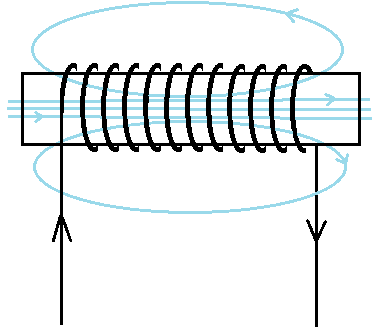
\includegraphics[scale=0.6]{electroaimant.png}
\caption{Modélisation d'un électroaimant}
\label{modélisation de l'électroaimant}
\end{figure}

Le nombre de spires de la bobine fixe, appelons-le $N_1$, a été choisi arbitrairement de manière à produire un
champ magnétique assez fort. Nous avons fixé ce nombre, selon les conseils de notre tuteur, à \numprint{420}. 
Nous allons maintenant calculer les caractéristiques suivantes de notre électroaimant :

\begin{itemize}
	\item Résistance totale de la bobine ;
	\item Champ magnétique induit ;
	\item Inductance.
\end{itemize}

\paragraph{Champ magnétique dans l'entrefer}
Pour céer un champ magnétique plus fort, nous avons réduit l'entrefer de $\unit{7}{\milli\meter}$.
Calculons dans un premier temps le champ magnétique dans l'entrefer de $\unit{7}{\milli\meter}$ en 
utilisant la conservation des flux. Pour ce calcul, nous utilisons l'hypothèse simplificatrice
assez forte que tout le champ se trouve dans l'entrefer.

$$H_e \cdot e = N_1 I \Rightarrow \frac{B_e}{\mu_0 \mu_r} e = N_1 I$$

Pour $N_1 = 420$, l'entrefer $e = \unit{0.007}{\meter}$, $\mu_r = 1.0000004$ la perméabilité magnétique
de l'air et $I = \unit{1}{\ampere}$, on trouve alors :

$B_e = \unit{0.07539825}{\tesla}$

\paragraph{Résistance totale de la bobine}
Pour calculer la résistance totale de la bobine, nous devons connaître la longueur totale de fil de cuivre utilisé.
Pour cela nous utilisons la formule suivante :

$$L{fil} = N_1 \cdot 2\pi r$$  

Où $N_1 = 420$ est le nombre de spires de la bobine fixe, et $r$ est la rayon des spires. Pour
$r = \unit{0.016}{\meter}$, on trouve :

$$L_{fil} = \unit{42.22}{\meter}$$

Il ne nous reste donc plus qu'à multiplier la longueur totale trouvée par la résistance linéique des fils de cuivre
($R_{lin} = \unit{0.18}{\ohm\per\meter}$) :

$$R = L_{fil} \cdot R_{lin} = \unit{7.6}{\ohm}$$

\paragraph{Inductance de la bobine}
Une fois le champ magnétique induit connu, l'inductance dans la bobine peut être très facilement calculée par :

$$L = N_1 \frac{\phi_B}{I}$$

Dans cette formule, il ne nous reste plus qu'à calculer $\phi_B = B \cdot A$ où $A = ab$ est l'aire d'une spire.
On trouve alors :

$L = \unit{0.025468}{\henry}$

\paragraph{Tableau récapitulatif}

\begin{center}
	\begin{tabular}{c|c|c|c|c}
		$N_1$ & $B_e$ & $R$ & $L$ & $L_{fil}$ \\
		\hline
		420 & $\unit{0.07539825}{\tesla}$ & \unit{7.6}{\ohm} & $\unit{0.0254683}{\henry}$ & $\unit{42.22}{\meter}$\\
	\end{tabular}
\end{center}

%Il faut encore recalculer la constante de raideur de la menbranne!

\subsection{Calcul de la constante de raideur de la membrane}
Avant de pouvoir déterminer le nombre de spires de la bobine mouvante, nous avons dû déterminer
expérimentalement la constante de raideur de notre papier pour faire la membrane.
Notre procédure a été la suivante: nous avons suspendu notre membrane, pour ensuite 
déposer un poids dessus, et finalement mesurer l'élongation du matériau.
Nous obtenons ainsi une constante de raideur d'environ \unit {80}{N/m}.

\subsection{Fonctionnement et dimensionnement de la bobine mobile}

\paragraph{Calcul du nombre de spires}
Etant donné que nous disposons d'un amplificateur qui, selon la datasheet, a une puissance de sortie de 
$\unit{2.5}{\watt}$, et que la tension de sortie est de $\unit{15}{\volt}$, nous pouvons trouver le courant
maximal passant dans la bobine mobile:

$$I = \frac{P}{V} = \unit{0.1667}{\ampere}$$

En fonction de la constante de raideur de la membrane trouvée dans la sous-section précédente et de l'écartement
maximal de la membrane par rapport à sa position d'origine (fixé à $d = \unit{0.003}{\meter}$), nous sommes en
mesure de trouver la longueur du fil de la bobine:

$$IL_{fil}B = kx$$
$$L_{fil} = \frac{kx}{IB} = 12.6 m$$

Le fil à notre disposition au laboratoire a un encombrement de $\unit{25.8}{\frac{spires}{cm}}$. Nous otenons 
donc une relation entre $N_2$, le nombre de spires, et $L_{bobine}$, la longueur de la bobine:

$$25.8 = \frac{N_2}{L_{bobine}}$$

En fixant le rayon à \unit{1.7}{mm}, nous pouvons déterminer $N_2$ ainsi que la longueur de la bobine:
$$L_{fil} = N_2 \cdot 2\pi r$$ 
$$N_2 =  \frac{L_{fil}}{2\pi r} = 118$$


\paragraph{Calcul de la résistance totale de la bobine mobile}
Pour calculer la résistance totale de la bobine, il ne nous reste plus qu'à multiplier la longueur de fil trouvée 
précédemment par la résistance linéique du fil de cuivre
($R_{lin} = \unit{0.18}{\ohm\per\meter}$) :

$$R = L_{fil} \cdot R_{lin} = \unit{2.38}{\ohm}$$

\paragraph{Calcul de l'inductance de la bobine mobile}

Une fois le champ magnétique induit connu, l'inductance dans la bobine peut être très facilement calculée par :

$$L = N_2 \frac{\phi_B}{I} = \unit{0.0734}{\henry}$$

\paragraph{Tableau récapitulatif}

\begin{center}
	\begin{tabular}{c|c|c|c}
		$N_2$ & $I$ & $R$ & $L$ \\
		\hline
		 $118$ & $\unit{0.1667}{\ampere}$ & $\unit{2.38}{\ohm}$ & $\unit{0.0734}{\henry}$ \\
	\end{tabular}
\end{center}

\begin{figure}[ht!]
\centering
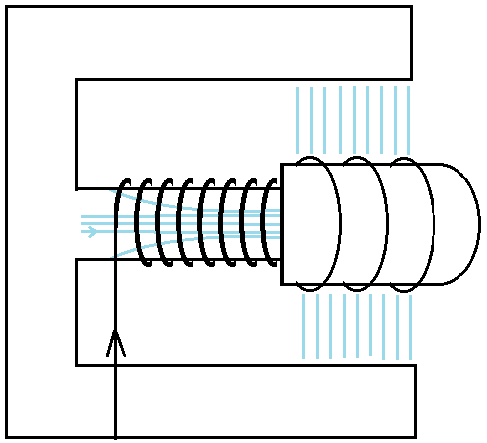
\includegraphics[scale=0.3]{hautparleur.png}
\caption{Vue d'ensemble avec la seconde bobine}
\label{Vue d'ensemble avec la seconde bobine}
\end{figure}

% Just here to fix rapport_prejury.tex
\end{document}

\chapter{Résultats des problèmes mathématiques}

\documentclass{article}

\usepackage[utf8]{inputenc}
\usepackage[T1]{fontenc}      
\usepackage[francais]{babel}
\usepackage{graphicx}
\usepackage{circuitikz}
\usepackage[squaren, Gray]{SIunits}
\usepackage{sistyle}
\usepackage[autolanguage]{numprint}
\usepackage{pgfplots}
\pgfplotsset{compat=1.9}
\usepackage{amsmath,amssymb,array}
\usepackage[top=2.5cm,bottom=2.5cm,right=2.5cm,left=2.5cm]{geometry}
\usepackage{url} 
\usepackage{tabularx}
\DeclareMathOperator{\dist}{d}
\newenvironment{abstract-fr}
{
	\begin{center}
		\textbf{Résumé} \\[0.5cm]
	\end{center}
}
{}

\newenvironment{abstract-en}
{
	\begin{center}
		\textbf{Summary} \\[0.5cm]
	\end{center}
}
{}
% New command pour la modélisation mécanique, tri à effectuer
\newcommand\fv[1]{{\bf #1}} % free vector
\newcommand\fvd[1]{\dot{\bf #1}} % free vector derivated
\newcommand\fvdd[1]{\ddot{\bf #1}} % free vector derivated
\newcommand\fvr[1]{\mathring{\bf #1}} % free vector relatively derivated
\newcommand\fvrr[1]{\overset{\circ\circ}{\bf #1}} % free vector relatively derivated
\newcommand\uv[1]{{\bf\hat{ #1}}} % unit vector
\newcommand\ui{{\bf\hat{I}}} % unit vector I
\newcommand\uj{{\bf\hat{J}}} % unit vector J
\newcommand\uk{{\bf\hat{K}}} % unit vector K
\newcommand\wrt[2]{\ensuremath{\tensor*[_{ #1}]{ #2}{}}} % With Respect To
\newcommand\wtr[3]{\ensuremath{\tensor*[_{ #1}]{ #2}{^{ #3}}}} % With Two Respect
\newcommand\omegaf{{\bm \omega}}
\newcommand\omegafr{\mathring{\bm \omega}}
\newcommand\omegafd{\dot{\bm \omega}}
\newcommand\omegaft{\tilde{\bm \omega}}
\newcommand\omegaftr{\mathring{\tilde{\bm \omega}}}
\newcommand\omegat{\tilde{\omega}}
\newcommand\omegatd{\tilde{\dot{\omega}}}
\newcommand\ine{{\bf I}}
\newcommand\st{{\bf L}}
\newcommand\pst{{\bf M}}
\newcommand\lm{{\bf N}}
\newcommand\am{{\bf H}}
\newcommand\amd{\dot{\am}}
\newcommand\fo{{\bf F}}
\newcommand\po{\mathcal{P}}
\newcommand\xg{\ensuremath{\fv{R}}}
\newcommand\xgd{\ensuremath{\fvd{R}}}
\newcommand\xgdd{\ensuremath{\fvdd{R}}}
\newcommand\dvec[1]{\dot{\vec{ #1}}}
\newcommand\ddvec[1]{\ddot{\vec{ #1}}}
\newcommand\qp{\dot{q}}
\newcommand\dqp{\Delta \dot{q}}
\usepackage{url} 
\usepackage{hyperref}
\hypersetup{
    colorlinks,
    citecolor=black,
    filecolor=black,
    linkcolor=black,
    urlcolor=black
}

\begin{document}

\section{Modélisation des filtres passe-haut, passe-bas, et passe-bande}
Dans cette section, nous allons expliquer la méthode que nous avons
utiliseé pour trouver une expression analytique de la tension de sortie 
dans un filtre passe-bas, ainsi que dans un filtre passe-haut. Nous 
étudierons également la combinaison de ces deux filtres: le passe-bande.

Nous avons en réalité utilisé deux méthodes différentes qui, heureusement, 
aboutissent à la même solution. La première méthode utilise ce que nous
avons appris au premier quadrimestre concernant les équations différentielles.
Cette méthode est plus longue et plus compliquée que la deuxième, c'est pourquoi
nous ne la décrirons pas ici.
La deuxième méthode utilise ce que nous avons appris au deuxième quadrimestre 
concernant les équations différentielles et les complexes. 

\subsection{Le filtre passe-bas}
Le filtre passe-bas dans notre haut-parleur a pour but de laisser
passer les basses fréquences et d'atténuer les plus hautes fréquences.

Soit $V_R$ la tension à travers la résistance $R$, $V_C$ la tension à travers
le condensateur $C$, $V_{in}$ la tension d'entrée et $V_{out}$ la tension de
sortie du filtre.

\begin{figure}[!htb]
	\centering
	\begin{circuitikz}
		\draw (0,0) node[ocirc] (A){};
		\draw (0,0) to [R=$R$] (2,0);
		\draw (2,0) to [short] (4,0);
		\draw (4,0) node[ocirc] (C){};
		\draw (2,0) to [C=$C$] (2,-2);
		\draw (2,-2) to [short] (4,-2);
		\draw (4,-2) node[ocirc] (D){};
		\draw (0,-2) to [short] (2,-2);
		\draw (0,-2) node[ocirc] (B){};
		\draw (A) to[open, v=$V_ {in}$] (B);
		\draw (C) to[open, v=$V_{out}$] (D);
	\end{circuitikz}
	\caption{Schéma électrique d'un filtre passe-bas}
	\label{lwp_scheme}
\end{figure}

Sur le circuit ci-dessus (Figure \ref{lwp_scheme}), nous pouvons utiliser la loi des tensions de Kirchhoff :

$$V_{in} = V_R + V_{out}$$

Notons $V$ l'amplitude de la tension d'entrée sinusoïdale, et $i(t)$ le courant
en fonction du temps : 

$$V \cdot \cos (\omega t) = R \cdot i(t) + V_C$$

Or, le courant $i(t)$ à travers un condensateur est donné par $C \frac{dV_C}{dt}$, 
l'équation devient alors une équation différentielle en la fonction inconnue $V_C (t)$ :

$$V \cdot \cos (\omega t) = RC\frac{dV_C}{dt}  + V_C$$

Nous pouvons réécrire cette équation de la manière suivante, où $y = V_C(t)$ :

$$RCy' + y = V \cdot \cos (\omega t)$$

Cette équation va être la base de la méthode qui suit. Nous utiliserons également
la condition initiale suivante :

$$y(0) = 0$$

\subsubsection{Résolution de l'équation différentielle}

Nous savons que $\cos (\omega t)$ est égal à la partie réelle de l'exponentielle
complexe $e^{\omega i t}$. Nous réécrivons alors l'équation différentielle de la
manière suivante :

$$RCy' + y = V \cdot e^{\omega i t}$$

Comme pour toute équation différentielle linéaire non-homogène, nous allons travailler
en deux étapes :

\paragraph{Recherche de la solution homogène}

Le polynôme caractéristique de l'équation homogène est :

$$RC \cdot x + 1 = 0$$

Nous obtenons alors $x = \frac{-1}{RC}$ comme racine, et nous trouvons donc comme solution homogène :

$$y_h(t) = A \cdot e^{\frac{-t}{RC}}$$

Où $A$ est une constante appartenant à l'ensemble des réels. % A confirmer, j'ai un doute.

\paragraph{Recherche de la solution particulière}

La solution particulière que nous recherchons est de la forme :

$$y_p(t) = \alpha \cdot e^{\omega i t}$$

Il nous reste donc à déterminer la constante complexe $\alpha$. Pour ce faire,
nous injectons dans l'équation de départ $y_p(t)$ et sa dérivée première. Nous trouvons 
alors :

$$\alpha = \frac{V(1-RC\omega i)}{1+R^2C^2\omega^2}$$

La solution particulière est donc :

$$y_p(t) = \frac{V(1-RC\omega i)}{1+R^2C^2\omega^2} \cdot e^{\omega i t}$$

\paragraph{Solution complète}

La solution finale $y(t)$ est égale à $y_h(t) + y_p(t)$ :

$$y(t) = A \cdot e^{\frac{-t}{RC}} + \frac{V(1-RC\omega i)}{1+R^2C^2\omega^2} \cdot e^{\omega i t}$$

En retransformant ensuite l'exponentielle complexe en sa forme trigonométrique et en ne
gardant que la partie réelle, nous obtenons :

$$y(t) = V_C(t) = \frac{V(\cos (\omega t) + RC\omega \sin (\omega t))}{1 + \omega^2R^2C^2} + A \cdot e^{\frac{-t}{RC}}$$

\paragraph{Élimination de la constante}

Il ne nous reste plus qu'à éliminer la constante $A$ en utilisant la condition initiale.
Nous trouvons enfin :

$$A = -\frac{V}{1 + \omega^2R^2C^2}$$                         

\paragraph{Conclusion}

La tension de sortie en fonction du temps est donc donnée par :

$$V_{out} = \frac{V}{1 + \omega^2R^2C^2} \cdot (\cos (\omega t) + RC\omega \sin (\omega t) - e^{\frac{-t}{RC}})$$

Nous pouvons ensuite réécrire cette formule de manière à faire apparaître
le déphasage de la tension de sortie par rapport à la tension d'entrée. En transformant
$y_p(t)$ en utilisant la notation exponentielle $|z|e^{\phi i}$ d'un couple de la forme 
$a+bi$ et en utilisant ensuite la notation trigonométrique d'une exponentielle complexe,
nous trouvons, après quelques simplifications et mises en évidence :

$$V_{out} = \frac{V}{\sqrt{1 + R^2\omega^2C^2}}
\left(-\frac{e^{\frac{-t}{RC}}}{\sqrt{1 + R^2\omega^2C^2}} + \cos(\arctan(-RC\omega) + \omega t)\right)
$$

Il apparaît donc que le déphasage entre $V_{out}$ et $V_{in}$ est $-\arctan(RC\omega) = -\arctan(2\pi fRC)$.
Ce déphasage augmente donc linéairement avec $\omega$ et est dû au temps que met le condensateur
à se charger. % A vérifier

\subsubsection{Vérification des résultats}

Une première vérification que l'on peut faire est de vérifier que $V_{out}$ tend vers \numprint{0}
lorsque $\omega$ tend vers l'infini. C'est bien le cas ici puisque $\omega^2$ est au dénominateur.

Nous pouvons ensuite regarder les graphes de $V_{out}$, $V_{in}$ (Figure \ref{lwp_voltages}) et $V_{out} / V_{in}$
(Figure \ref{lwp_ratio}). Les résultats sont encourageants.

\begin{figure}[!htb]
	\centering
	\begin{tikzpicture}[>=stealth]
    \begin{axis}[
        xmin=0,xmax=6,
        ymin=-8,ymax=8,
        axis x line=middle,
        axis y line=middle,
        axis line style=->,
        xlabel={$V$},
        ylabel={$t$},
        ]
				
        \addplot[no marks,black,-] expression[domain=0:6,samples=1000]
						{((7.5)/(sqrt(1 + 1000^2 * 0.00001^2 * 400^2))) * (((-2.718^((-x)/(1000*0.00001)))/(sqrt(1 + 1000^2 * 0.00001^2 * 400^2))) 
						+ cos(atan(-1000*0.00001*400) + 400*x))} 
						node[pos=0.65,anchor=south west]{$$};
						
				\addplot[no marks,blue,-] expression[domain=0:6,samples=1000]
						{7.5 * cos(400 * x)} 
						node[pos=0.65,anchor=south west]{$$}; 

    \end{axis}
	\end{tikzpicture}
	\caption{Graphe de $V_{out}$ (en noir) et $V_{in}$ (en bleu) pour les valeurs suivantes : $V_{max} = \unit{7.5}{\volt}$, $C = \unit{0.00001}{\farad}$,
						$R = \unit{1000}{\ohm}$ et $f = \unit{63.66}{\hertz}$}
	\label{lwp_voltages}
\end{figure}

\begin{figure}[!htb]
	\centering
	\begin{tikzpicture}[>=stealth]
    \begin{axis}[
        xmin=0,xmax=1400,
        ymin=0,ymax=1.2,
        axis x line=middle,
        axis y line=middle,
        axis line style=->,
        xlabel={$f$},
        ylabel={$V_{out} / V_{in}$},
        ]
				
				\addplot[no marks,green,-] expression[domain=0:1400,samples=100]
						% Formule par rapport aux expressions obtenues, un peu décallée
						% {(((7.5)/(sqrt(1 + 100^2 * 0.00001^2 * (2*3.14*x)^2))) * (((-2.718^((-100*0.00001)/(100*0.00001)))/(sqrt(1 + 100^2 * 
						% 0.00001^2 * (2*3.14*x)^2))) + cos(atan(-100*0.00001*2*3.14*x) + 2*3.14*x*100*0.00001)))/(7.5 * cos(2*3.14*x*100*0.00001))}
						{(1 + (2*3.14*x*100*0.00001)^2)^(-0.5)}
						node[pos=0.65,anchor=south west]{$$}; 
    \end{axis}
	\end{tikzpicture}
	\caption{Graphe de $V_{out} / V_{in} = \frac{1}{\sqrt{1 + (RC\omega)^2}}$ pour les valeurs suivantes : $R = \unit{100}{\ohm}$ et $C = {\unit{0.00001}{\farad}}$.}
	\label{lwp_ratio}
\end{figure}

\bigbreak

\subsection{Le filtre passe-haut}
Le filtre passe-haut a le rôle inverse du filtre passe-bas : il atténue les
basses fréquences et laisse passer les hautes fréquences.

Soit $V_R$ la tension à travers la résistance $R$, $V_C$ la tension à travers
le condensateur $C$, $V_{in}$ la tension d'entrée et $V_{out}$ la tension de
sortie du filtre.

\begin{figure}[!htb]
	\centering
	\begin{circuitikz}
		\draw (0,0) node[ocirc]{} (A);
		\draw (0,0) to [C=$C$] (2,0);
		\draw (2,0) to [short] (4,0);
		\draw (4,0) node[ocirc]{} (C);
		\draw (2,0) to [R=$R$] (2,-2);
		\draw (2,-2) to [short] (4,-2);
		\draw (4,-2) node[ocirc]{} (D);
		\draw (0,-2) to [short] (2,-2);
		\draw (0,-2) node[ocirc]{} (B);
		\draw (A) to[open, v=$V_ {in}$] (B);
		\draw (C) to[open, v=$V_{out}$] (D);
	\end{circuitikz}
	\caption{Schéma électrique d'un filtre passe-haut.}
	\label{hgp_scheme}
\end{figure}

Sur la Figure \ref{hgp_scheme}, la loi des tensions de Kirchhoff donne la même équation que pour le filtre passe-bas :

$$V_{in} = V_R + V_C$$

Cette fois, $V_{out} = V_R$. Or, nous connaissons déjà $V_C$ que nous avons calculé dans
le section précédente. Nous avons alors simplement :

$$V_R = V_{in} - V_C$$

$$V_{out} = \frac{V}{\sqrt{1 + R^2\omega^2C^2}}
\left(\frac{e^{\frac{-t}{RC}}}{\sqrt{1 + R^2\omega^2C^2}} - \cos(\arctan(-RC\omega) + \omega t) \right) + \cos(\omega t)$$

Le déphasage reste donc le même que pour le filtre passe-bas.

\subsubsection{Vérification des résultats}

Pour le filtre passe-haut, nous allons cette fois vérifier que lorsque $\omega$ tend vers \numprint{0}, nous avons
$V_{out}$ qui tend vers \numprint{0} également. Une fois de plus, c'est bien le cas.

Nous pouvons ensuite comparer les graphes de $V_{out}$, $V_{in}$ (Figure \ref{hgp_voltages}) et $V_{out} / V_{in}$
(Figure \ref{hgp_ratio}). Le déphasage apparaît clairement, et les fréquences les plus basses sont effectivement atténuées.

\begin{figure}[!htb]
	\centering
	\begin{tikzpicture}[>=stealth]
    \begin{axis}[
        xmin=0,xmax=6,
        ymin=-8,ymax=8,
        axis x line=middle,
        axis y line=middle,
        axis line style=->,
        xlabel={$V$},
        ylabel={$t$},
        ]
				
        \addplot[no marks,black,-] expression[domain=0:6,samples=1000]
						{(7.5 * cos(100*x)) - ((7.5)/(sqrt(1 + 1000^2 * 0.00001^2 * 100^2))) * (((-2.718^((-x)/(1000*0.00001)))/(sqrt(1 + 1000^2 *
						0.00001^2 * 100^2))) + cos(atan(-1000*0.00001*100) + 100*x))} 
						node[pos=0.65,anchor=south west]{$V_{out}$};
						
				\addplot[no marks,blue,-] expression[domain=0:25,samples=1000]
						{7.5 * cos(100 * x)} 
						node[pos=0.65,anchor=south west]{$V_{in}$}; 
				
    \end{axis}
	\end{tikzpicture}
	\caption{Graphe de $V_{out}$ et $V_{in}$ pour les valeurs suivantes : $V_{max} = \unit{7.5}{\volt}$, $C = \unit{0.00001}{\farad}$,
					$R = \unit{1000}{\ohm}$ et $f = \unit{15.91}{\hertz}$}
	\label{hgp_voltages}
\end{figure}

\begin{figure}[!htb]
	\centering
	\begin{tikzpicture}[>=stealth]
    \begin{axis}[
        xmin=0,xmax=1400,
        ymin=0,ymax=1,
        axis x line=middle,
        axis y line=middle,
        axis line style=->,
        xlabel={$f$},
        ylabel={$V_{out}/V_{in}$},
        ]

				\addplot[no marks,green,-] expression[domain=0:1400,samples=100]
				% Formule obtenue avec nos expressions, décallée de 0.4 vers le haut.
				%		{((7.5 * cos(2*3.14*x*100*0.00001)) - ((7.5)/(sqrt(1 + 100^2 * 0.00001^2 * (2*3.14*x)^2))) * 		
				%	(((-2.718^((-100*0.00001)/(100*0.00001)))/(sqrt(1 + 100^2 *0.00001^2 * (2*3.14*x)^2))) + cos(atan(-100*0.00001*2*3.14*x) +
				%	2*3.14*x*100*0.00001)))/(7.5 * cos(2*3.14*x*100*0.00001))}
				{(1 + (1)/((2*3.14*x*100*0.00001)^2))^(-0.5)}
						node[pos=0.65,anchor=south west]{$$}; 

    \end{axis}
	\end{tikzpicture}
	\caption{Graphe de $V_{out} / V_{in} = 1 + \frac{1}{{\sqrt{1+(RC\omega)^2}}}$ pour les valeurs suivantes : $R = \unit{100}{\ohm}$ et $C = {\unit{0.0001}{\farad}}$.}
	\label{hgp_ratio}
\end{figure}

\bigbreak

\subsection{Le filtre passe-bande}
Le filtre passe-bande sert, comme son nom l'indique, à laisser passer une certaine
bande de fréquence. Il est constitué d'un filtre passe-haut suivi d'un passe-bas.
Les fréquences de coupure respectives des filtres déterminent 
l'ampleur de la bande passante. Plus la résistance pour le filtre passe-bas 
(resp.passe-haut) est petite (resp.grande), plus la bande passante est large, 
étant donné que la fréquence de coupure est inversément proportionnelle à la 
résistance. 

Soit $V_{in,1}$ la tension à l'entrée du filtre passe-bas, $R_{1}$ la résistance, 
et $C_{1}$ la capacité. Dans la section précédente, nous sommes arrivés au résultat suivant :

$$V_{out,1} = \frac{V_{in,1}}{\sqrt{1 + R_{1}^2\omega^2C_{1}^2}}
\left (-\frac{e^{\frac{-t}{R_{1}C_{1}}}}{\sqrt{1 + R_{1}^2\omega^2C_{1}^2}} + \cos(\arctan(-R_{1}C_{1}\omega) + \omega t)\right)$$

Cette tension de sortie du filtre passe-bas sera notre tension d'entrée pour le 
filtre passe-haut. Précédemment, dans la section concernant le filtre passe-haut,
nous trouvions :

$$V_{out,2} = \frac{V_{in,2}}{\sqrt{1 + R_{2}^2\omega^2C_{2}^2}}
\left(\frac{e^{\frac{-t}{R_{2}C_{2}}}}{\sqrt{1 + R_{2}^2\omega^2C_{2}^2}} - 
\cos(\arctan(-R_{2}C_{2}\omega) + \omega t)\right) + V_{in,2}\cos(\omega t)$$

où $V_{in,2}$ est la tension à l'entrée du filtre passe-haut, $R_{2}$ la résistance, 
et $C_{2}$ la capacité. Étant donné que nous disposons d'un adaptateur d'impédance, 
nous pouvons nous permettre d'utiliser ces deux équations obtenues séparément.
En remplaçant $V_{in,2}$ par $V_{out,1}$, la tension à la sortie du passe-bas, nous 
trouvons $V_{out,3}$, la tension de sortie finale.
Après simplifications, nous obtenons :

$$V_{out,3} = \frac{V_{out,1} \cdot V_{out,2}}{V_{in,1}}$$

\begin{figure}[ht!]
	\centering
	\begin{tikzpicture}[>=stealth]
			\begin{axis}[
					xmin=0,xmax=2000,
					ymin=0,ymax=1.2,
					axis x line=middle,
					axis y line=middle,
					axis line style=->,
					xlabel={$f$},
					ylabel={$V_{out} / V_{in}$},
					legend entries = {passe-bande, fréq. coupure 1, fréq. coupure 2}
					]

					\addplot[no marks,red,-] expression[domain=0:2000,samples=100]
					{(((2*3.14*x*10000*0.00000047)*(1 + (2*3.14*x*10000*0.00000047)^2)^(-0.5))*
					((1 + (2*3.14*x*500*0.00000047)^2)^(-0.5)))};
					\addplot[no marks, gray] coordinates
					{(33.86,0) (33.86,1.1)};
					\addplot[no marks, gray] coordinates
					{(677.26,0) (677.26,1.1)};
		\end{axis}
	\end{tikzpicture}
	\caption{Graphe de $V_{out} / V_{in}$ pour le filtre passe-bande, pour les valeurs
	suivantes: $R_{1} = \unit{500}{\ohm}$, $R_{2} = \unit{10000}{\ohm}$, et 
	$C = {\unit{0.00000047}{\farad}}$}
	\label{pbf_ratio}
\end{figure}

\subsubsection{Vérification des résultats}

Au vu du graphe de $V_{out,3} / V_{in,1}$ de l'équation obtenue pour le passe-bande, nous pouvons
valider notre résultat, étant donné que l'allure du graphique sur la Figure \ref{pbf_ratio} correspond à nos attentes. En effet,
les fréquences de coupure théoriques représentées sur la figure semblent concorder avec les courbes.

% Just here to fix rapport_prejury.tex
\end{document}


\documentclass{report}


\usepackage[latin1]{inputenc}
\usepackage[T1]{fontenc}
\usepackage[francais]{babel}
\usepackage{amsmath,amssymb,array}
 
      
\title{Résultats filtre passe-haut et passe-bas}
\author{Groupe 11.53}
\date{fevrier 2014}
\begin{document}
 
\maketitle

\chapter{Passe-bas}
\section{Equation de la droite horizontale}

Nous savons que la droite a une valeur initiale de 2.5 V et donc \[y=2.5\]

\section{Equation de la droite diagonale}

Nous savons que l'équation de la droite est de type $y=a*x+b$
\\
Mais pour cette situation-ci, nous allons utiliser une base logarithmique pour la pente.  En effet, les différentes fréquences utilisées sont tellement éloignées les unes des autres que le graphique serait gigantesque et la pente diagonale serait en fait une courbe.  Ce qui donne: $y=a*\log{x}+b$


Voici 3 résultats mesurés en laboratoire.
\bigbreak
\\
\begin{tabular}{|c|c|c|}
\hline
V_c & f & log{ f} \\
\hline
1.7 & 16000 & 4.204\\
\hline
1.55 & 18000 & 4.255\\
\hline
1.45 & 20000 & 4.301 \\
\hline
\end{tabular}

\bigbreak
Des maintenant les fréquences sont exprimées en base logarithmique et nous obtenons la matrice suivante:
\bigbreak
$$
\begin{pmatrix}  
 4.204 & 1\\
 4.255 & 1 \\
 4.301 & 1 
\end{pmatrix}
\begin{pmatrix}  
a\\
b
\end{pmatrix}
=
\begin{pmatrix}  
1.7\\
1.55\\
1.45
\end{pmatrix}
$$
\bigbreak

Ce qui nous donne les vecteurs suivants:

\[e_1=( \frac{1}{\sqrt[]{3}} \frac{1}{\sqrt[]{3}} \frac{1}{\sqrt[]{3}})\]

\\ et

\\
\[e_2=( -0.68, 0.03, 0.73)\]

\bigbreak
Ce qui nous donne une projection de 
$$
\begin{pmatrix}  
1.6\\
1.5\\
1.4
\end{pmatrix}$$
$$

\bigbreak
Nous en déduisons la valeur des coefficients a et b:  
\[ a =-1.96 \]
\[ b= 9.84 \]

$$\fbox{y= -1.96 \timeslog{x} +9.84}$$

\bigbreak
Pour trouver la fréquence d'intersection entre les deux droites $$y=2.5$$ et $$y= -1.96 \times log{x} +9.84$$ nous égalisons les y et nous trouvons $$\fbox{x=5557.7 Hz$$} 

\\
Cela nous semble correct car en théorie nous devons arriver à une valeur f tel que $$f=\frac{1}{2\times \pi\times R\times C}$$
avec $R=7.5+50=57.5 ohms$ et $C=470\times 10^{-9} F$  Notre valeur théorique de la fréquence est donc $$f=5889.2 Hz$$


\chapter{Passe-haut}

\section{Equation de la droite horizontale}

Nous savons que la droite a une valeur initiale de 0.75 V et donc \[y=0.75\]

\section{Equation de la droite diagonale}

Nous savons que l'équation de la droite est de type $y=a*x+b$
\\
Mais pour cette situation-ci, nous allons utiliser une base logarithmique pour la pente.  En effet, les différentes fréquences utilisées sont tellement éloignées les unes des autres que le graphique serait gigantesque et la pente diagonale serait en fait une courbe.  Ce qui donne: $y=a*\log{x}+b$


Voici 3 résultats mesurés en laboratoire.
\bigbreak
\\
\begin{tabular}{|c|c|c|}
\hline
V_c & f & log{ f} \\
\hline
127 & 0.4 & 2.1\\
\hline
191 & 0.5 & 2.3\\
\hline
356 & 0.6 & 2.6 \\
\hline
\end{tabular}

\bigbreak
Des maintenant les fréquences sont exprimées en base logarithmique et nous obtenons la matrice suivante:
\bigbreak
$$
\begin{pmatrix}  
 2.1 & 1\\
 2.3 & 1 \\
 2.6 & 1 
\end{pmatrix}
\begin{pmatrix}  
a\\
b
\end{pmatrix}
=
\begin{pmatrix}  
0.4\\
0.5\\
0.6
\end{pmatrix}
$$
\bigbreak

Ce qui nous donne les vecteurs suivants:

\[e_1=( \frac{1}{\sqrt[]{3}} \frac{1}{\sqrt[]{3}} \frac{1}{\sqrt[]{3}})\]

\\ et

\\
\[e_2=( -0.6, 0, 0.8)\]

\bigbreak
Ce qui nous donne une projection de 
$$
\begin{pmatrix}  
0.36\\
0.5\\
0.69
\end{pmatrix}$$
$$

\bigbreak
Nous en déduisons la valeur des coefficients a et b:  
\[ a =0.7 \]
\[ b= -1.11 \]

$$\fbox{y= -1.96 \timeslog{x} +9.84}$$

\bigbreak
Pour trouver la fréquence d'intersection entre les deux droites $$y=0.75$$ et $$y= 0.7 \times log{x} -1.11$$ nous égalisons les y et nous trouvons $$\fbox{x=439.4 Hz$$} 




\end{document}


\chapter{Recherches documentaires}

\documentclass{article}

\usepackage[utf8]{inputenc}
\usepackage[T1]{fontenc}      
\usepackage[francais]{babel}
\usepackage{graphicx}
\usepackage{circuitikz}
\usepackage[squaren, Gray]{SIunits}
\usepackage{sistyle}
\usepackage[autolanguage]{numprint}
\usepackage{pgfplots}
\pgfplotsset{compat=1.9}
\usepackage{amsmath,amssymb,array}
\usepackage[top=2.5cm,bottom=2.5cm,right=2.5cm,left=2.5cm]{geometry}
\usepackage{url} 
\usepackage{tabularx}
\DeclareMathOperator{\dist}{d}
\newenvironment{abstract-fr}
{
	\begin{center}
		\textbf{Résumé} \\[0.5cm]
	\end{center}
}
{}

\newenvironment{abstract-en}
{
	\begin{center}
		\textbf{Summary} \\[0.5cm]
	\end{center}
}
{}
% New command pour la modélisation mécanique, tri à effectuer
\newcommand\fv[1]{{\bf #1}} % free vector
\newcommand\fvd[1]{\dot{\bf #1}} % free vector derivated
\newcommand\fvdd[1]{\ddot{\bf #1}} % free vector derivated
\newcommand\fvr[1]{\mathring{\bf #1}} % free vector relatively derivated
\newcommand\fvrr[1]{\overset{\circ\circ}{\bf #1}} % free vector relatively derivated
\newcommand\uv[1]{{\bf\hat{ #1}}} % unit vector
\newcommand\ui{{\bf\hat{I}}} % unit vector I
\newcommand\uj{{\bf\hat{J}}} % unit vector J
\newcommand\uk{{\bf\hat{K}}} % unit vector K
\newcommand\wrt[2]{\ensuremath{\tensor*[_{ #1}]{ #2}{}}} % With Respect To
\newcommand\wtr[3]{\ensuremath{\tensor*[_{ #1}]{ #2}{^{ #3}}}} % With Two Respect
\newcommand\omegaf{{\bm \omega}}
\newcommand\omegafr{\mathring{\bm \omega}}
\newcommand\omegafd{\dot{\bm \omega}}
\newcommand\omegaft{\tilde{\bm \omega}}
\newcommand\omegaftr{\mathring{\tilde{\bm \omega}}}
\newcommand\omegat{\tilde{\omega}}
\newcommand\omegatd{\tilde{\dot{\omega}}}
\newcommand\ine{{\bf I}}
\newcommand\st{{\bf L}}
\newcommand\pst{{\bf M}}
\newcommand\lm{{\bf N}}
\newcommand\am{{\bf H}}
\newcommand\amd{\dot{\am}}
\newcommand\fo{{\bf F}}
\newcommand\po{\mathcal{P}}
\newcommand\xg{\ensuremath{\fv{R}}}
\newcommand\xgd{\ensuremath{\fvd{R}}}
\newcommand\xgdd{\ensuremath{\fvdd{R}}}
\newcommand\dvec[1]{\dot{\vec{ #1}}}
\newcommand\ddvec[1]{\ddot{\vec{ #1}}}
\newcommand\qp{\dot{q}}
\newcommand\dqp{\Delta \dot{q}}
\usepackage{url} 
\usepackage{hyperref}
\hypersetup{
    colorlinks,
    citecolor=black,
    filecolor=black,
    linkcolor=black,
    urlcolor=black
}

\begin{document}

\section{La contre-réaction ou réaction négative}
En analysant le circuit de notre haut-parleur, nous avons découvert la présence de boucle reliant la sortie et la borne négative des amplificateurs. Nous nous sommes alors interrogés sur le rôle de ces boucles.

Nous allons dans un premier temps expliquer les raisons d'être des boucles de contre-réaction en général et nous finirons par l'explication complète de leur raison d'être dans le cas particulier de notre circuit.

\subsection{Principe de la réaction}
Le principe de la réaction est présent dans un grand nombre de circuits électroniques. Il consiste en une réinjection d'une partie du signal de sortie à l'entrée du circuit pour le combiner avec le signal d'entrée extérieur.

Il existe deux types de réactions :

\begin{itemize}
	\item \textbf{La réaction positive} : le signal réinjecté est en phase avec le signal d'entrée de telle sorte que les deux signaux s'additionnent ;
	\item \textbf{La réaction négative} (ou contre-réaction) : le signal réinjecté est en opposition de phase avec le signal d'entrée, de telle sorte que les deux signaux
	se soustraient.
\end{itemize}

\begin{figure}[h]
	\centering
	\begin{circuitikz}
		\draw (0, 0) node[ocirc];
		\draw (0, 0)	to[short] (2, 0);
		\draw (0, -1) node[ocirc];
		\draw (0, -1) to[short] (2, -1);
		\draw (3.1, -0.5) node [op amp, yscale=-1.022] (op amp) {}
					(opamp.-)node[left]
					(opamp.+)node[left]
					(opamp.out)node[right];
		\draw (3.85, -0.5) to[short] (5.6, -0.5);
		\draw (5.6, -0.5) node[ocirc];
		\draw (5.4, -0.5) to[short] (5.4, -2);
		\draw (5.4, -2) to[short] (1.4, -2);
		\draw (1.4, -2) to[short] (1.4, -1);
	\end{circuitikz}
	\caption{Schéma électrique d'une boucle de réaction sur un 	amplificateur.}
	\label{reaction1}
\end{figure}

\subsection{Effets des boucles de contre-réaction}

\subsubsection{En général}
Les effets des boucles de contre-réaction sur un amplificateur sont nombreux :

\begin{itemize}
	\item La boucle de contre-réaction rend indépendant le gain de l'amplificateur des différentes variations du circuits ;
	\item Le signal de sortie est plus proche du signal d'entrée que si l'amplificateur avait été en boucle ouverte ;
	\item Réduction des signaux électriques parasites et de la distorsion dûs à l'amplificateur : en boucle ouverte, le taux de distorsion d'un amplificateur est typiquement de 1\%. La boucle de contre-réaction permet de diminuer ce taux à 0.001\% ;
	\item Contrôle du gain de l'amplificateur (qui est, en boucle ouverte, de l'ordre de $10^6$) ;
	\item Elargissement de la bande passante de l'amplificateur ;
	\item Réduction de l'impédance de sortie.
\end{itemize}

\subsubsection{Dans notre cas particulier}
Dans notre cas particulier, le principal effet de la boucle de contre-réaction est le contrôle du gain de l'amplificateur qui ramène à $1$ le gain.

\begin{figure}[h]
	\centering
	\begin{circuitikz}
		\draw (0,0) node[ocirc];
		\draw (3,0) to[short] (opamp+);
		\draw (4, -0.5) node [op amp, yscale=-1.022] (op amp) {}
			(opamp.-)node[left] (opamp-)
			(opamp.+)node[left] (opamp+)
			(opamp.out)node[right] (opampout);
		\draw (5, -0.5) to[short] (7, -0.5);
		\draw (7, -0.5) node[ocirc];
		\draw (2, -1) to[short] (3, -1);
		\draw (2, -1) to[short] (2, -3);
		\draw (2, -3) to[R=$R_1$] (2, -4);
		\draw (2, -4) to[short] (2, -4.5);
		\draw (2, -4) node[ground];
		\draw (2, -2) to[short] (6, -2);
		\draw (6, -2) to[R=$R_2$] (6, -0.5);
	\end{circuitikz}
	\caption{Schéma électrique d'une boucle de réaction sur un 	amplificateur avec un diviseur résistif.}
	\label{reaction2}
\end{figure}

Sur la Figure \ref{reaction2}, on remarque que la tension de sortie et la tension d'entrée sont liées par la formule des diviseurs résistifs :

$$V_{in} = \frac{R_1}{R_1 + R_2} V_{out}$$

Le gain est alors donné par :

$$A = \frac{V_{out}}{V_{in}} = \frac{R_1 + R_2}{R_1}$$

Pour réduire le gain $A$ à $1$, on a alors deux possibilités :

\begin{enumerate}
	\item	Choisir $R_1 >> R_2$ ;
	\item Choisir $R_2 = 0$ ;
\end{enumerate}

La possibilité la plus simple est la deuxième, car en choississant $R_2 = 0$, le gain est donné par $\frac{R_1}{R_1}$. Autrement dit : quelque soit $R_1$, on a $A = 1$ de telle sorte que $V_{in} = V_{out}$. On choisi alors $R_1$ si petit que le remplacer par un simple court-circuit a le même effet.

Dans un tel montage (appelé \texit{suiveur de tension}), la résistance d'entrée est infinie alors que la résistance de sortie est faible. Le courant de sortie est alors plus grand que le courant d'entrée (qui est presque nul).

\nocite{*} 
\bibliographystyle{plain}
\bibliography{source}

% Just here to fix rapport_prejury.tex
\end{document}

\documentclass{article}

\usepackage[utf8]{inputenc}
\usepackage[T1]{fontenc}      
\usepackage[francais]{babel}
\usepackage{graphicx}
\usepackage{circuitikz}
\usepackage[squaren, Gray]{SIunits}
\usepackage{sistyle}
\usepackage[autolanguage]{numprint}
\usepackage{pgfplots}
\pgfplotsset{compat=1.9}
\usepackage{amsmath,amssymb,array}
\usepackage[top=2.5cm,bottom=2.5cm,right=2.5cm,left=2.5cm]{geometry}
\usepackage{url} 
\usepackage{tabularx}
\DeclareMathOperator{\dist}{d}
\newenvironment{abstract-fr}
{
	\begin{center}
		\textbf{Résumé} \\[0.5cm]
	\end{center}
}
{}

\newenvironment{abstract-en}
{
	\begin{center}
		\textbf{Summary} \\[0.5cm]
	\end{center}
}
{}
% New command pour la modélisation mécanique, tri à effectuer
\newcommand\fv[1]{{\bf #1}} % free vector
\newcommand\fvd[1]{\dot{\bf #1}} % free vector derivated
\newcommand\fvdd[1]{\ddot{\bf #1}} % free vector derivated
\newcommand\fvr[1]{\mathring{\bf #1}} % free vector relatively derivated
\newcommand\fvrr[1]{\overset{\circ\circ}{\bf #1}} % free vector relatively derivated
\newcommand\uv[1]{{\bf\hat{ #1}}} % unit vector
\newcommand\ui{{\bf\hat{I}}} % unit vector I
\newcommand\uj{{\bf\hat{J}}} % unit vector J
\newcommand\uk{{\bf\hat{K}}} % unit vector K
\newcommand\wrt[2]{\ensuremath{\tensor*[_{ #1}]{ #2}{}}} % With Respect To
\newcommand\wtr[3]{\ensuremath{\tensor*[_{ #1}]{ #2}{^{ #3}}}} % With Two Respect
\newcommand\omegaf{{\bm \omega}}
\newcommand\omegafr{\mathring{\bm \omega}}
\newcommand\omegafd{\dot{\bm \omega}}
\newcommand\omegaft{\tilde{\bm \omega}}
\newcommand\omegaftr{\mathring{\tilde{\bm \omega}}}
\newcommand\omegat{\tilde{\omega}}
\newcommand\omegatd{\tilde{\dot{\omega}}}
\newcommand\ine{{\bf I}}
\newcommand\st{{\bf L}}
\newcommand\pst{{\bf M}}
\newcommand\lm{{\bf N}}
\newcommand\am{{\bf H}}
\newcommand\amd{\dot{\am}}
\newcommand\fo{{\bf F}}
\newcommand\po{\mathcal{P}}
\newcommand\xg{\ensuremath{\fv{R}}}
\newcommand\xgd{\ensuremath{\fvd{R}}}
\newcommand\xgdd{\ensuremath{\fvdd{R}}}
\newcommand\dvec[1]{\dot{\vec{ #1}}}
\newcommand\ddvec[1]{\ddot{\vec{ #1}}}
\newcommand\qp{\dot{q}}
\newcommand\dqp{\Delta \dot{q}}
\usepackage{url} 
\usepackage{hyperref}
\hypersetup{
    colorlinks,
    citecolor=black,
    filecolor=black,
    linkcolor=black,
    urlcolor=black
}

\begin{document}

\section{La distorsion harmonique}

La distorsion est un critère de qualité en ce qui concerne les haut-parleurs.
Dans le soucis de construire un dispositif de qualité, nous avons décidé de 
nous informer sur la distorsion harmonique, un concept que nous ne connaissions
que de nom.
Ce document est structuré comme suit: nous parlerons tout d'abord de la notion  de distorsion 
en général pour ensuite aborder la notion  de distorsion 
harmonique, et finalement décrire ses causes, ses effets,
et les moyens de diminution.

\subsection{Définition}
Commençons tout d'abord par comprendre la notion de distorsion du son: par définition, c'est
une transformation du signal audio par rapport à celui de sortie. Une distorsion n'est généralement pas vraiment souhaitée, étant donné
que le signal en est déformé. Cependant, certains audiophiles en tirent avantage, vu que que quelques
transformations peuvent mener à un son plus chaud et agréable.

\paragraph{La distorsion harnomique}
La distorsion harmonique joue sur la superposition de différentes fréquences:
la fréquence fondamentale et ses harmoniques. Un haut-parleur parfait émettrait seulement la fréquence fondamentale, sans les harmoniques, qui sont donc des "parasites".
On parle d'harmonique pour désigner les multiples entiers de la fréquence fondamentale.
Par exemple, la seconde harmonique d'une fréquence de 50 Hz vaut 100Hz, la troisième 150Hz, etc. La figure 
ci-dessous illustre adéquatement cette notion.
Les harmoniques paires sont les moins incommodantes, étant donné qu'elles représentent la même note, mais à quelques octaves de différence.
Les harmoniques impaires, elles, sont plus gênantes étant donné que la note est différente.

\begin{figure}[h]
\centering
\includegraphics[scale=0.6]{image2.png}
\caption{Superposition d'une fréquence fondamentale et de ses premières hamoniques.}
\label{Superposition d'une fréquence fondamentale et de ses premières hamoniques.}
\end{figure}

\subsection{Causes}
À cause de la distorsion harmonique, le signal que nous faisons circuler dans notre haut-parleur n'est pas
une sinusoïdale parfaite mais plutôt une série de Fourier, c'est-à-dire une somme de sinusoïdes de 
fréquence et d'amplitude différentes. C'est l'appareil en lui-même qui crée la distorsion, étant donné 
qu'il ne reproduit généralement pas parfaitement le signal d'entrée. 
Les charges non-linéaires sont les principales causes de distorsion harmonique. Celles-ci causent 
l'apparition des courants harmoniques qui sont eux-mêmes responsables de la distorsion harmonique.

\subsection{Conséquences}
La distorsion harmonique a plusieurs conséquences néfastes.
La plus importante de toutes vient du fait que les harmoniques impaires génèrent un son dur, et peu agréable. De plus, la distorsion cause un accroissement 
du courant dans un système. Il va en résulter une surchauffe des composantes électriques (conducteurs, 
capacités,...). À la longue, des disfonctionnements non souhaités peuvent provoquer un vieillissement 
précoce du circuit électrique. Il existe de nombreuses autres conséquences néfastes, mais n'oublions pas de préciser que certaines personnes recherchent tout de même ces distorsions pour produire un son plus agréable, au moyen d'harmoniques paires.

\subsection{Solutions}
Pour éviter toute distorsion, ou tout simplement pour émettre un son plus pur et exact, 
il existe différentes solutions. Nous parlerons seulement des filtres actifs 
mais il est intéressant de savoir que d'autre moyens tels que les selfs AC ou DC, ainsi que les redresseurs
multi-pulses, existent. 
Les filtres actifs permettent d'éliminer les harmoniques perturbatrices en injectant des courants
harmoniques de mêmes fréquences mais déphasés d'une demi-période. Cela cause des interférences
destructrices avec les harmoniques dont on souhaite se débarrasser. La résultante est une droite constante
nulle n'influençant pas notre signal.

\nocite{*}
\bibliographystyle{plain}
\bibliography{source}

% Just here to fix rapport_prejury.tex
\end{document}

\part{Conclusion}

\clearpage

\nocite{*} 
\bibliographystyle{plain}
\bibliography{../../sources/sources}

\part{Annexes}
\appendix

\documentclass{article}

\usepackage[utf8]{inputenc}
\usepackage[T1]{fontenc}      
\usepackage[francais]{babel}
\usepackage{graphicx}
\usepackage{circuitikz}
\usepackage[squaren, Gray]{SIunits}
\usepackage{sistyle}
\usepackage[autolanguage]{numprint}
\usepackage{pgfplots}
\pgfplotsset{compat=1.9}
\usepackage{amsmath,amssymb,array}
\usepackage[top=2.5cm,bottom=2.5cm,right=2.5cm,left=2.5cm]{geometry}
\usepackage{url} 
\usepackage{tabularx}
\DeclareMathOperator{\dist}{d}
\newenvironment{abstract-fr}
{
	\begin{center}
		\textbf{Résumé} \\[0.5cm]
	\end{center}
}
{}

\newenvironment{abstract-en}
{
	\begin{center}
		\textbf{Summary} \\[0.5cm]
	\end{center}
}
{}
% New command pour la modélisation mécanique, tri à effectuer
\newcommand\fv[1]{{\bf #1}} % free vector
\newcommand\fvd[1]{\dot{\bf #1}} % free vector derivated
\newcommand\fvdd[1]{\ddot{\bf #1}} % free vector derivated
\newcommand\fvr[1]{\mathring{\bf #1}} % free vector relatively derivated
\newcommand\fvrr[1]{\overset{\circ\circ}{\bf #1}} % free vector relatively derivated
\newcommand\uv[1]{{\bf\hat{ #1}}} % unit vector
\newcommand\ui{{\bf\hat{I}}} % unit vector I
\newcommand\uj{{\bf\hat{J}}} % unit vector J
\newcommand\uk{{\bf\hat{K}}} % unit vector K
\newcommand\wrt[2]{\ensuremath{\tensor*[_{ #1}]{ #2}{}}} % With Respect To
\newcommand\wtr[3]{\ensuremath{\tensor*[_{ #1}]{ #2}{^{ #3}}}} % With Two Respect
\newcommand\omegaf{{\bm \omega}}
\newcommand\omegafr{\mathring{\bm \omega}}
\newcommand\omegafd{\dot{\bm \omega}}
\newcommand\omegaft{\tilde{\bm \omega}}
\newcommand\omegaftr{\mathring{\tilde{\bm \omega}}}
\newcommand\omegat{\tilde{\omega}}
\newcommand\omegatd{\tilde{\dot{\omega}}}
\newcommand\ine{{\bf I}}
\newcommand\st{{\bf L}}
\newcommand\pst{{\bf M}}
\newcommand\lm{{\bf N}}
\newcommand\am{{\bf H}}
\newcommand\amd{\dot{\am}}
\newcommand\fo{{\bf F}}
\newcommand\po{\mathcal{P}}
\newcommand\xg{\ensuremath{\fv{R}}}
\newcommand\xgd{\ensuremath{\fvd{R}}}
\newcommand\xgdd{\ensuremath{\fvdd{R}}}
\newcommand\dvec[1]{\dot{\vec{ #1}}}
\newcommand\ddvec[1]{\ddot{\vec{ #1}}}
\newcommand\qp{\dot{q}}
\newcommand\dqp{\Delta \dot{q}}
\usepackage{url} 
\usepackage{hyperref}
\hypersetup{
    colorlinks,
    citecolor=black,
    filecolor=black,
    linkcolor=black,
    urlcolor=black
}

\begin{document}

\section{Projet specifications}

\begin{table*} [h]

\begin{tabular}{|l|c|l|}

\hline
&&\\
\textbf{Group} & & \hfill \textbf{Date}  March 7th 2014\\
11.53 && \hfill \textbf{Version} 2.1\\

\hline
\multicolumn{3}{|p{15cm}|}{\textbf{Context} \newline
Our goal during this project is to realize, qualify, and measure an amplification system. This device should allow us to hear smartphone signals from two loudspeakers. The volume and the intensity of the bass and treble sounds should be adjustable.}  \\


\hline
\textbf{Date} & \textbf{Origine} & \textbf{Content}\\
\hline
&&\\
&&\textbf{Principal functions}\\
&&\\
16/02/14 & Costumer & 1. Emit a sound \\
16/02/14 & Costumer & 2. Amplify a sound \\
16/02/14 & Costumer & 3. Variation of bass and treble \\
&&\\
\hline
&&\\
& & \textbf{Criteria and level of the main functions} \\
&&\\
16/02/14 & Group & 1.1. Sound between ... and... Hz \\
16/02/14 & Costumer & 2.1. Power of 2.5 W \\
&&\\
\hline
&&\\
& & \textbf{Constraints} \\
&&\\
16/02/14 & Costumer &   Jackplug of 3.5 mm in diameter\\
16/02/14 & Laboratory &  Input voltage of 30V \\
07/03/14 & Costumer&  Paper membrane \\
&&\\
\hline
&&\\
& & \textbf{Terms} \\
&&\\
07/03/14 & Group & Type of paper : 200 g/m$^{2}$ \\
07/03/14 & Group & Cost estimation : ...\\

&&\\
\hline
\end{tabular}

\end{table*}

\end{document}


\bigbreak

\documentclass{article}

\usepackage[utf8]{inputenc}
\usepackage[T1]{fontenc}      
\usepackage[francais]{babel}
\usepackage{graphicx}
\usepackage{circuitikz}
\usepackage[squaren, Gray]{SIunits}
\usepackage{sistyle}
\usepackage[autolanguage]{numprint}
\usepackage{pgfplots}
\pgfplotsset{compat=1.9}
\usepackage{amsmath,amssymb,array}
\usepackage[top=2.5cm,bottom=2.5cm,right=2.5cm,left=2.5cm]{geometry}
\usepackage{url} 
\usepackage{tabularx}
\DeclareMathOperator{\dist}{d}
\newenvironment{abstract-fr}
{
	\begin{center}
		\textbf{Résumé} \\[0.5cm]
	\end{center}
}
{}

\newenvironment{abstract-en}
{
	\begin{center}
		\textbf{Summary} \\[0.5cm]
	\end{center}
}
{}
% New command pour la modélisation mécanique, tri à effectuer
\newcommand\fv[1]{{\bf #1}} % free vector
\newcommand\fvd[1]{\dot{\bf #1}} % free vector derivated
\newcommand\fvdd[1]{\ddot{\bf #1}} % free vector derivated
\newcommand\fvr[1]{\mathring{\bf #1}} % free vector relatively derivated
\newcommand\fvrr[1]{\overset{\circ\circ}{\bf #1}} % free vector relatively derivated
\newcommand\uv[1]{{\bf\hat{ #1}}} % unit vector
\newcommand\ui{{\bf\hat{I}}} % unit vector I
\newcommand\uj{{\bf\hat{J}}} % unit vector J
\newcommand\uk{{\bf\hat{K}}} % unit vector K
\newcommand\wrt[2]{\ensuremath{\tensor*[_{ #1}]{ #2}{}}} % With Respect To
\newcommand\wtr[3]{\ensuremath{\tensor*[_{ #1}]{ #2}{^{ #3}}}} % With Two Respect
\newcommand\omegaf{{\bm \omega}}
\newcommand\omegafr{\mathring{\bm \omega}}
\newcommand\omegafd{\dot{\bm \omega}}
\newcommand\omegaft{\tilde{\bm \omega}}
\newcommand\omegaftr{\mathring{\tilde{\bm \omega}}}
\newcommand\omegat{\tilde{\omega}}
\newcommand\omegatd{\tilde{\dot{\omega}}}
\newcommand\ine{{\bf I}}
\newcommand\st{{\bf L}}
\newcommand\pst{{\bf M}}
\newcommand\lm{{\bf N}}
\newcommand\am{{\bf H}}
\newcommand\amd{\dot{\am}}
\newcommand\fo{{\bf F}}
\newcommand\po{\mathcal{P}}
\newcommand\xg{\ensuremath{\fv{R}}}
\newcommand\xgd{\ensuremath{\fvd{R}}}
\newcommand\xgdd{\ensuremath{\fvdd{R}}}
\newcommand\dvec[1]{\dot{\vec{ #1}}}
\newcommand\ddvec[1]{\ddot{\vec{ #1}}}
\newcommand\qp{\dot{q}}
\newcommand\dqp{\Delta \dot{q}}
\usepackage{url} 
\usepackage{hyperref}
\hypersetup{
    colorlinks,
    citecolor=black,
    filecolor=black,
    linkcolor=black,
    urlcolor=black
}

\begin{document}

\section{Méthode de recherche}

\subsection{La contre-réaction ou réaction négative}
Comme suggeré lors de la séance d'information sur la recherche bibliographique,
nous avons appliqué la méthode de l'entonnoir. Comme les boucles de contre-réaction 
sont directement %liées aux amplificateurs, nous avons commencé nos recherche avec 
les termes plutôt généraux : \textit{amplificateurs} et \textit{amplifiers}. Nous 
nous avons ensuite associé à ces %mots clés les termes plus précis : \textit{contre-réaction}
et \textit{negative feedback}.

Les différents ouvrages et documents que nous avons utilisés sont listés dans la bibliographie

\subsection{La distorsion harmonique}

\paragraph{Choix du thème}
Le choix du thème n'a pas été chose aisée. Nous avons commencé par établir un brainstorming afin de réunir 
le plus d'idée possibles. Cependant, les thèmes proposés nous semblaient trop généraux que pour faire un vrai 
travail en profondeur tout en restant concis. Quelqu'un a finalement proposé la distorsion harmonique; un 
terme visible sur les emballages de haut-parleurs. Curieux d'en apprendre plus sur ce terme presque méconnu, 
nous avons décidé de débuter notre travail de recherche là-dessus.

\paragraph{Recherche documentaire}
Etant donné que nous ne connaissions vraiment que très peu sur ce sujet et que nous 
le devions comprendre en profondeur, nous avons commencé par le terme général de "distorsion".
Une première recherche sur internet a permis de fixer les idées à propos de ce terme, et nous 
avons ensuite pu établir une liste de mot-clefs pour entamer réellement la recherche sur la 
distorsion harmonique. Nous avons appliqué la "technique de l'entonnoir", et nous %avons finalement 
réuni assez d'informations que pour écrire ce rapport. Notons tout de même que c'est indiscutablement
en anglais que nous avons 
trouvé le plus d'informations. Nous avons gardé une trace de toutes les sources que nous avons 
consultées, et cela a rendu l'écriture de la bibliographie nettement plus facile.

% Just here to fix rapport_prejury.tex
\end{document}

%\input{../../constante_raideur/constante_raideur}

\end{document}
